% Using template for a Computer Science Tripos Part II project dissertation
\documentclass[12pt,a4paper,twoside,openright]{report}
\usepackage[pdfborder={0 0 0}]{hyperref}    % turns references into hyperlinks
\usepackage[margin=25mm]{geometry}  % adjusts page layout
\usepackage{graphicx}  % allows inclusion of PDF, PNG and JPG images
\usepackage{verbatim}
\usepackage{docmute}   % only needed to allow inclusion of proposal.tex

\raggedbottom                           % try to avoid widows and orphans
\sloppy
\frenchspacing
\clubpenalty1000%
\widowpenalty1000%

\renewcommand{\baselinestretch}{1.1}    % adjust line spacing to make
                                        % more readable

\begin{document}

\bibliographystyle{plain}


%%%%%%%%%%%%%%%%%%%%%%%%%%%%%%%%%%%%%%%%%%%%%%%%%%%%%%%%%%%%%%%%%%%%%%%%
% Title


\pagestyle{empty}

\rightline{\LARGE \textbf{Z\'ebulon Goriely}}

\vspace*{60mm}
\begin{center}
\Huge
\textbf{Simulating Language Learning and Evolution} \\[5mm]
Computer Science Tripos -- Part II \\[5mm]
Queens' College \\[5mm]
\today  % today's date
\end{center}

%%%%%%%%%%%%%%%%%%%%%%%%%%%%%%%%%%%%%%%%%%%%%%%%%%%%%%%%%%%%%%%%%%%%%%%%%%%%%%
% Proforma, table of contents and list of figures

\pagestyle{plain}

\chapter*{Proforma}

{\large
\begin{tabular}{ll}
Name:               & \bf Z\'ebulon Goriely                       \\
College:            & \bf Queens' College                     \\
Project Title:      & \bf Simulating Language Learning and Evolution \\
Examination:        & \bf Computer Science Tripos -- Part II, May 2020  \\
Word Count:         & \bf NULL\footnotemark[1]  \\
Project Originator: & Z\'ebulon Goriely                    \\
Supervisor:         & Prof. Paula Buttery and Dr. Andrew Caines                  \\ 
\end{tabular}
}
\footnotetext[1]{This word count was computed
by \texttt{detex diss.tex | tr -cd '0-9A-Za-z $\tt\backslash$n' | wc -w}
}
\stepcounter{footnote}


\section*{Original Aims of the Project}

To write a demonstration dissertation\footnote{A normal footnote without the
complication of being in a table.} using \LaTeX\ to save
student's time when writing their own dissertations. The dissertation
should illustrate how to use the more common \LaTeX\ constructs. It
should include pictures and diagrams to show how these can be
incorporated into the dissertation.  It should contain the entire
\LaTeX\ source of the dissertation and the makefile.  It should
explain how to construct an MSDOS disk of the dissertation in
Postscript format that can be used by the book shop for printing, and,
finally, it should have the prescribed layout and format of a diploma
dissertation.


\section*{Work Completed}

All that has been completed appears in this dissertation.

\section*{Special Difficulties}

Learning how to incorporate encapulated postscript into a \LaTeX\
document on both Ubuntu Linux and OS X.
 
\newpage
\section*{Declaration}

I, Z\'ebulon Goriely of Queens' College, being a candidate for Part II of the Computer
Science Tripos, hereby declare
that this dissertation and the work described in it are my own work,
unaided except as may be specified below, and that the dissertation
does not contain material that has already been used to any substantial
extent for a comparable purpose.

\bigskip
\leftline{Signed Z\'ebulon Goriely}

\medskip
\leftline{Date [date]}

\tableofcontents

\listoffigures

\newpage
\section*{Acknowledgements}

This document owes much to an earlier version written by Simon Moore
\cite{Moore95}.  His help, encouragement and advice was greatly 
appreciated.

%%%%%%%%%%%%%%%%%%%%%%%%%%%%%%%%%%%%%%%%%%%%%%%%%%%%%%%%%%%%%%%%%%%%%%%
% now for the chapters

\pagestyle{headings}

\chapter{Introduction}

\section{Overview of the files}

This document consists of the following files:

\begin{itemize}
\item \texttt{makefile} --- The makefile for the dissertation and
                         Project Proposal
\item \texttt{diss.tex} --- The dissertation
\item \texttt{proposal.tex}  --- The project proposal 
\item \texttt{figs} -- A directory containing diagrams and pictures
\item \texttt{refs.bib} --- The bibliography database
\end{itemize}

\section{Building the document}

This document was produced using \LaTeXe which is based upon
\LaTeX\cite{Lamport86}.  To build the document you first need to
generate \texttt{diss.aux} which, amongst other things, contains the
references used.  This if done by executing the command:

\texttt{pdflatex diss}

\noindent
Then the bibliography can be generated from \texttt{refs.bib} using:

\texttt{bibtex diss}

\noindent
Finally, to ensure all the page numbering is correct run \texttt{pdflatex}
on \texttt{diss.tex} until the \texttt{.aux} files do not change.  This
usually takes 2 more runs.

\subsection{The makefile}

To simplify the calls to \texttt{pdflatex} and \texttt{bibtex}, 
a makefile has been provided, see Appendix~\ref{makefile}. 
It provides the following facilities:

\begin{description}

\item\texttt{make} \\
 Display help information.

\item\texttt{make proposal.pdf} \\
 Format the proposal document as a PDF.

\item\texttt{make view-proposal} \\
 Run \texttt{make proposal.pdf} and then display it with a Linux PDF viewer
 (preferably ``okular'', if that is not available fall back to ``evince'').

\item\texttt{make diss.pdf} \\
 Format the dissertation document as a PDF.

\item\texttt{make count} \\
Display an estimate of the word count.

\item\texttt{make all} \\
Construct \texttt{proposal.pdf} and \texttt{diss.pdf}.

\item\texttt{make pub} \\ Make \texttt{diss.pdf}
and place it in my \texttt{public\_html} directory.

\item\texttt{make clean} \\ Delete all intermediate files except the
source files and the resulting PDFs. All these deleted files can
be reconstructed by typing \texttt{make all}.

\end{description}


\section{Counting words}

An approximate word count of the body of the dissertation may be
obtained using:

\texttt{wc diss.tex}

\noindent
Alternatively, try something like:

\verb/detex diss.tex | tr -cd '0-9A-Z a-z\n' | wc -w/


\chapter{Preparation}

This chapter is empty!


\chapter{Implementation}

\section{Verbatim text}

Verbatim text can be included using \verb|\begin{verbatim}| and
\verb|\end{verbatim}|. I normally use a slightly smaller font and
often squeeze the lines a little closer together, as in:

{\renewcommand{\baselinestretch}{0.8}\small
\begin{verbatim}
GET "libhdr"
 
GLOBAL { count:200; all  }
 
LET try(ld, row, rd) BE TEST row=all
                        THEN count := count + 1
                        ELSE { LET poss = all & ~(ld | row | rd)
                               UNTIL poss=0 DO
                               { LET p = poss & -poss
                                 poss := poss - p
                                 try(ld+p << 1, row+p, rd+p >> 1)
                               }
                             }
LET start() = VALOF
{ all := 1
  FOR i = 1 TO 12 DO
  { count := 0
    try(0, 0, 0)
    writef("Number of solutions to %i2-queens is %i5*n", i, count)
    all := 2*all + 1
  }
  RESULTIS 0
}
\end{verbatim}
}

\section{Tables}

\begin{samepage}
Here is a simple example\footnote{A footnote} of a table.

\begin{center}
\begin{tabular}{l|c|r}
Left      & Centred & Right \\
Justified &         & Justified \\[3mm]
%\hline\\%[-2mm]
First     & A       & XXX \\
Second    & AA      & XX  \\
Last      & AAA     & X   \\
\end{tabular}
\end{center}

\noindent
There is another example table in the proforma.
\end{samepage}

\section{Simple diagrams}

Simple diagrams can be written directly in \LaTeX.  For example, see
figure~\ref{latexpic1} on page~\pageref{latexpic1} and see
figure~\ref{latexpic2} on page~\pageref{latexpic2}.

\begin{figure}
\setlength{\unitlength}{1mm}
\begin{center}
\begin{picture}(125,100)
\put(0,80){\framebox(50,10){AAA}}
\put(0,60){\framebox(50,10){BBB}}
\put(0,40){\framebox(50,10){CCC}}
\put(0,20){\framebox(50,10){DDD}}
\put(0,00){\framebox(50,10){EEE}}

\put(75,80){\framebox(50,10){XXX}}
\put(75,60){\framebox(50,10){YYY}}
\put(75,40){\framebox(50,10){ZZZ}}

\put(25,80){\vector(0,-1){10}}
\put(25,60){\vector(0,-1){10}}
\put(25,50){\vector(0,1){10}}
\put(25,40){\vector(0,-1){10}}
\put(25,20){\vector(0,-1){10}}

\put(100,80){\vector(0,-1){10}}
\put(100,70){\vector(0,1){10}}
\put(100,60){\vector(0,-1){10}}
\put(100,50){\vector(0,1){10}}

\put(50,65){\vector(1,0){25}}
\put(75,65){\vector(-1,0){25}}
\end{picture}
\end{center}
\caption{A picture composed of boxes and vectors.}
\label{latexpic1}
\end{figure}

\begin{figure}
\setlength{\unitlength}{1mm}
\begin{center}

\begin{picture}(100,70)
\put(47,65){\circle{10}}
\put(45,64){abc}

\put(37,45){\circle{10}}
\put(37,51){\line(1,1){7}}
\put(35,44){def}

\put(57,25){\circle{10}}
\put(57,31){\line(-1,3){9}}
\put(57,31){\line(-3,2){15}}
\put(55,24){ghi}

\put(32,0){\framebox(10,10){A}}
\put(52,0){\framebox(10,10){B}}
\put(37,12){\line(0,1){26}}
\put(37,12){\line(2,1){15}}
\put(57,12){\line(0,2){6}}
\end{picture}

\end{center}
\caption{A diagram composed of circles, lines and boxes.}
\label{latexpic2}
\end{figure}



\section{Adding more complicated graphics}

The use of \LaTeX\ format can be tedious and it is often better to use
encapsulated postscript (EPS) or PDF to represent complicated graphics.
Figure~\ref{epsfig} and~\ref{xfig} on page \pageref{xfig} are
examples. The second figure was drawn using \texttt{xfig} and exported in
{\tt.eps} format. This is my recommended way of drawing all diagrams.


\begin{figure}[tbh]
\centerline{
\includegraphics{figs/cuarms.pdf}}
\caption{Example figure using encapsulated postscript}
\label{epsfig}
\end{figure}

\begin{figure}[tbh]
\vspace{4in}
\caption{Example figure where a picture can be pasted in}
\label{pastedfig}
\end{figure}


\begin{figure}[tbh]
\centerline{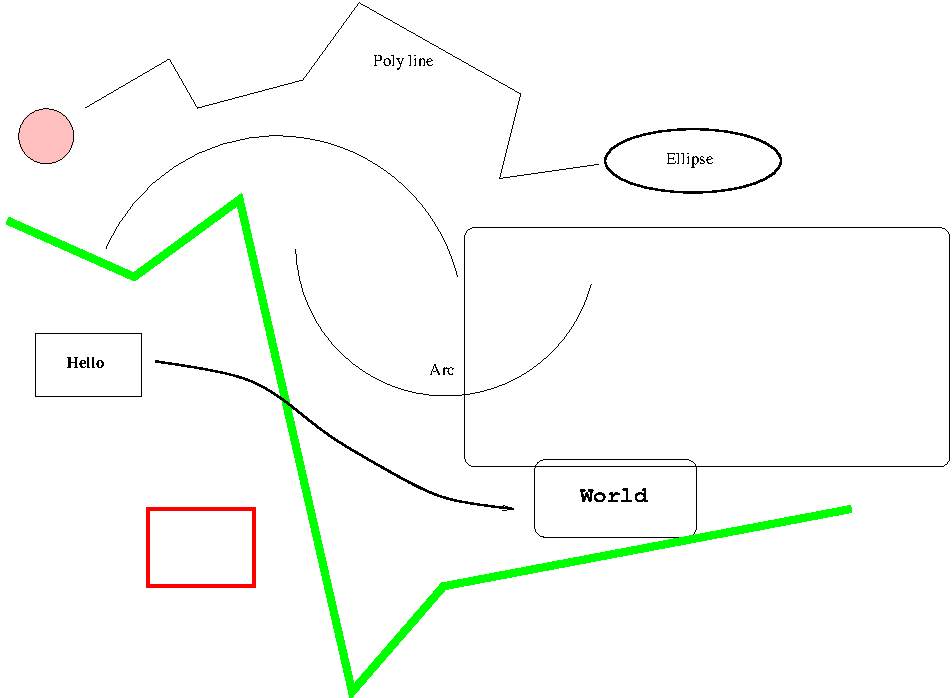
\includegraphics{figs/diagram.pdf}}
\caption{Example diagram drawn using \texttt{xfig}}
\label{xfig}
\end{figure}


\chapter{Evaluation}

\section{Printing and binding}

Use a ``duplex'' laser printer that can print on both sides to print
two copies of your dissertation. Then bind them, for example using the
comb binder in the Computer Laboratory Library.

\section{Further information}

See the Unix Tools notes at

\url{http://www.cl.cam.ac.uk/teaching/current-1/UnixTools/materials.html}


\chapter{Conclusion}

I hope that this rough guide to writing a dissertation is \LaTeX\ has
been helpful and saved you time.


%%%%%%%%%%%%%%%%%%%%%%%%%%%%%%%%%%%%%%%%%%%%%%%%%%%%%%%%%%%%%%%%%%%%%
% the bibliography
\addcontentsline{toc}{chapter}{Bibliography}
\bibliography{refs}

%%%%%%%%%%%%%%%%%%%%%%%%%%%%%%%%%%%%%%%%%%%%%%%%%%%%%%%%%%%%%%%%%%%%%
% the appendices
\appendix

\chapter{Latex source}

\section{diss.tex}
{\scriptsize\verbatiminput{diss.tex}}

\section{proposal.tex}
{\scriptsize\verbatiminput{proposal.tex}}

\chapter{Makefile}

\section{makefile}\label{makefile}
{\scriptsize\verbatiminput{makefile.txt}}

\section{refs.bib}
{\scriptsize\verbatiminput{refs.bib}}


\chapter{Project Proposal}

\documentclass[12pt]{article}
\usepackage{a4wide}
\usepackage{datetime}
\usepackage{url}
\usepackage{hyperref}
\usepackage[svgnames]{xcolor}
\hypersetup{
  colorlinks,
  urlcolor=Blue}

\newcommand{\al}{$<$}
\newcommand{\ar}{$>$}
\newcommand{\sups}{\textsuperscript}
\newcommand{\belgianspacing}{\frenchspacing}

\parindent 0pt
\parskip 6pt

\begin{document}

\belgianspacing

\thispagestyle{empty}

%\rightline{\large\emph{Z\'ebulon Goriely}}
%\medskip
%\rightline{\large\emph{Queens'}}
%\medskip
%\rightline{\large\emph{zg258}}

%\vfil

\centerline{\large Computer Science Part II Project Proposal}
\vspace{0.2in}
\centerline{\Large\bf Simulating Language Learning and Evolution}
\vspace{0.2in}
\centerline{\large {\bf{Z\'ebulon Goriely --- Queens' --- zg258}}}
\vspace{0.2in}
\newdate{proposaldate}{18}{10}{2019}
\centerline{\large {\displaydate{proposaldate}}}
 
 \vspace{0.3in}
 
%\vfil

{\bf Project Originator:} Z\'ebulon Goriely

{\bf Project Supervisor:} {Prof. Paula Buttery and Dr. Andrew Caines}

{\bf Director of Studies:}  {Prof. Alastair Beresford}

{\bf Overseers:} {Prof. Pietro Lio’} and {Dr. Robert Mullins}

\section*{Introduction}

Language has evolved and therefore probably gave an evolutionary advantage to the individuals that exhibited it. As Angelo Cangelosi and Domenico Parisi described in a 1998 paper\footnote{\url{https://doi.org/10.1080/095400998116512}}, it is difficult to investigate the evolutionary origin of language and the selective pressures that may have originated language due to the limited evidence available. They propose using computer simulations of evolutionary scenarios to investigate this. In the paper referenced, they describe a simulated toy world where agents controlled by neural-networks interact with an environment of mushrooms that are edible and poisonous. This simulation and the ideas explored in the paper will be the basis for my project.

In the paper, Cangelosi and Parisi use small feed-forward neural networks to control the behaviour of each agent. The weights are initially random; a genetic algorithm is used to improve the fitness of the species over many generations. The agents are also given linguistic abilities; input and output nodes of the neural networks produce signals that allow for communication.

By creating three different populations (one without language, one with an externally imposed language and one with an evolved language) we can investigate the evolutionary advantage of language. Furthermore, it allows us to investigate a key question posed in the paper: \emph{``Since language requires the parallel evolution of linguistic production and linguistic comprehension, how can language evolve when it has a purely informative function and therefore it is advantageous to the receiver but not the producer?''}

For this project, I will re-implement the simulation described. I will then create analysis tools to investigate the findings of the paper to see if I observe the same results.

\section*{Starting Point}

I have a small amount of experience in programming simulations; for my A-Level project in 2016, I created a simulation of virus propogation between mosquito and human agents in the Unity game engine.

I do not have any experience programming neural networks, however, I am confident that I understand the backpropagation algorithm and basic neural network structure through the Artificial Intelligence course I took last year. In the papers I plan to reference, Cangelosi very clearly describes the structure of the neural networks he uses and I am confident that I will be able to follow his work.

Over the summer I read a book titled Simulating the Evolution of Language which gave me an overview of the techniques used in this field. Alongside the Formal Models of Language course that I took last year, I now have a sufficient base of understanding to begin this project.

\section*{Work to be Done}

The work for this project can be roughly divided into two stages; implementing the simulation and constructing the means of evaluating my implementation against the findings in the original paper. I will also regularly be creating tests to evaluate my simulation.

\subsection*{Implementing the Simulation}

\begin{enumerate}

\item Set up the simulation environment by creating the world grid and implementing the properties of poisonous and edible mushrooms. Create the simulation loop divided into regular `epochs'.

\item Create the agents for the simulation, giving them position and energy properties.

\item Implement feedforward neural networks to control the behaviour of the agents; input units to identify the location of the nearest mushroom, visual perception units to observe mushroom properties (only when close enough) and signal perception units for when language is implemented. The output units control the movement of the agent and production of signals. There will also be hidden units.

\item Implement the genetic algorithm that runs after all agents complete the simulation. The fittest agents are determined by the energy level (based on eating edible mushrooms and avoiding poisonous mushrooms). The fittest agents are then chosen for asexual reproduction, producing offspring that have genetic mutations in the form selecting a percentage of the weights to change by a random amount.

\item Create two different populations, one without language (where the signal perception units are always set to the same, constant value) and one with an externally imposed language (where the signal perception units are set to one of two signals depending on the type of the nearest mushroom).

\item Create a third population with an evolved language. Instead of externally imposed signals, in each simulation cycle one of the other agents is randomly selected as the `speaker' and its output is connected to the input signal perception units of the `listener'. 

\end{enumerate}

\subsection*{Analysis}

\begin{enumerate}

\item Plot the average fitness over the number of generations to compare between the three populations.

\item Produce some behavioural tests to investigate the behaviour of random individual organisms at specific generations.

\item Plot the frequency distribution of the different signals produced by the individuals with the evolved language using a `naming task'.

\item Calculate the Quality Index (QI) of the language produced by the population without language and the population with an evolved language to investigate the genetic advantage of producing productive signals. The QI evaluates the efficiency of a language based off of three criteria; (1) functionally distinct categories are labeled with distinct signals, (2) a single signal tends to be used to label all the instances within a category and (3) all the individuals in the population tend to use the same signal to label the same category.

\item Investigate the correlation between QI of the language and the fitness of the species to determine if change in the language or in the categorisation skill of the agents affects the other ability.

\end{enumerate}

\subsection*{Testing}

To evaluate my project and ensure that my simulation implementation is functional, I will create an ensemble of unit tests for each of the tasks above. These will be created in parallel as I develop each part of the implementation. For the simulation, this will involve small examples or scenarios to show that each part of the simulation is fully functional.

\section*{Success Criterion}

The project will be deemed a success if I can implement the simulation as described in the tasks above (evaluated by my unit tests) and if I can implement the analysis tools to compare the findings of my implementation to the findings of the original paper.

\section*{Timetable and Milestones}

I've broken down this timetable into two and three week intervals. At the end of December, I will be writing my Progress Report and simultaneously making adjustments to the timetable as needed.

\subsection*{25\sups{th} October -- 10\sups{th} November}

\emph{Middle of Michaelmas Term. Includes first deadline for NLP coursework.}


{\bf Task:} Create a high-level design of the system. Set up the project files with a version-control system. Experiment with creating small simulations in python and do suitable research into Neural Network libraries.

{\bf Milestones:} Have a git repository with project files. Have a design plan with specific details of the simulation confirmed.

\subsection*{11\sups{th} November -- 24\sups{th} November}

\emph{Middle of Michaelmas Term.}


{\bf Task:} Complete implementation tasks 1 and 2 as described above. Experiment with adding Neural Networks to control the behaviour of the agents.

{\bf Milestones:} Have a working simulation environment with poisonous and edible mushrooms. Have agents with positions and energy values but no functional neural networks yet.

\subsection*{25\sups{th} November -- 8\sups{th} December}

\emph{End of Michaelmas Term. Includes second and third deadline for NLP coursework.}


{\bf Task:} Complete implementation tasks (3). Start working on implementation task (4).

{\bf Milestones:} Have the agents successfully controlled by neural networks. Be able to run an entire lifespan of one agent within the simulated world. Have the beginnings of a 

\subsection*{9\sups{th} December -- 22\sups{nd} December}

\emph{Christmas holiday. Will likely be in Cambridge to help with Queens' interviews.}

{\bf Task:} Complete implementation tasks (4), (5) and (6). Also aim to complete analysis tasks (1) and (3).

{\bf Milestones:} Have a fully functional simulation that allows for running a thousand generations of a population of agents. Have three different populations to compare; one without language, one with an externally imposed language and one with an evolved language. Have a tool to graph the average fitness of each population over the number of generations and another tool to view the probability distribution of the signals chosen for the evolved language over the number of generations.

\subsection*{23\sups{rd} December -- 12\sups{th} January}

\emph{Christmas holiday. Will take a break to revise Michaelmas courses and to spend time with family.}

{\bf Task:} Complete analysis task (2). Write the Preparation chapter of the Dissertation. Review the timetable for the remainder of the project and adjust in light of experience so far. If ahead of schedule, plan time for extensions. Start to plan tests cases.

{\bf Milestones:} An outline of the dissertation document with a completed Preparation section.

\subsection*{13\sups{th} January -- 2\sups{nd} February}

\emph{Start of Lent term. Will have regular labs for Mobile Robot Systems.}

{\bf Progress Report Deadline:} 31\sups{st} January

{\bf Task:} Write the Progress Report. Start to fill out the Implementation chapter of the Dissertation. Complete analysis tasks (4) and (5).

{\bf Milestones:} Progress report submitted and entired project reviewed both personally and with overseers. Have tools to plot the Quality Index of the evolved language against the fitness of the population. At this point, all the tasks in the {\bf Work to Do} section will have been completed, satisfying the {\bf Success Criteria}.

\subsection*{3\sups{rd} February -- 23\sups{rd} February}

\emph{Middle of Lent term. Both deadlines for the Mobile Robot Systems assignments.}

{\bf Task:} Begin analysis of the simulation. Begin to work on extensions to the project, keeping in mind time needed to write the Dissertation.

{\bf Milestones:} Have the start of a test suite with a series of diagrams to use to evaluate my implementation.

\subsection*{24\sups{th} February -- 15\sups{th} March}

\emph{End of Lent term. Deadline for the Mobile Robot Systems mini-project report.}

{\bf Task:} Complete testing. Evaluate the outcomes of the tests against the findings in the original paper. At this point, the second half of the {\bf Success Criteria} will have been achieved. If needed, revise the implementation to be clean, documented and consise. Work on other extensions.

{\bf Milestones:} Examples and test cases run with results collected. Code should perform a variety of interesting tasks and should be in a state that in the worst case it would satisfy the examiners with at most cosmetic adjustment

\subsection*{16\sups{th} March -- 5\sups{th} April}

\emph{Start of Easter holiday. Might stay in Cambridge for part of it to work. Will balance revision and work on the project.}

{\bf Task:} Complete work on any extensions. Draft the Evaluations and Conclusions chapters of the Dissertation.

{\bf Milestones:} Extensions almost complete. Skeleton of entire Dissertation in place.

\subsection*{6\sups{th} April -- 19\sups{th} April}

\emph{End of Easter holiday. Might get back to Cambridge early to work. Will balance revision and work on the project.}

{\bf Task:} Complete the Implementation and Introduction chapters of the Dissertation. Send the full draft to Director of Studies and Supervisors by 21st of April.

{\bf Milestones:} Dissertation essentially complete, with large sections of it proof-read by Supervisors and possibly friends and/or Director of Studies.

\subsection*{20\sups{th} April -- 8\sups{th} May}

\emph{Start of Easter Term. Will be balancing revision, lectures and final work on the project.}

{\bf Final Deadline:} 8\sups{th} May

{\bf Task:} Finish Dissertation, preparing diagrams for insertion. Review the whole project, checking the Dissertation and spending the final few days on whatever is in greatest need of attention. Aim to submit the dissertation at least a week before the deadline.

{\bf Milestone:} Submission of Dissertation

\section*{Possible Extensions}

\subsection*{Graphic Visualisation}

As a side extension, I could implement a visual interface to watch the life of one agent within the simulation. This would involve rendering a simple 2D world with textures for the agents and mushrooms. This could be expanded further by adding a User Interface for setting up the simulation and having windows showing the progress as it occurs live.

\subsection*{Symbolic Theft vs. Sensorimotor Toil}

In a 2000 paper\footnote{\url{http://cogprints.org/2036/}}, Cangelosi and Harnad use a similar same toy world of mushrooms and foragers to place two ways of acquiring categories in direct competition with each other. They compare ``sensorimotor toil'' (where categories are acquired through real-time, feedback-correct, trial and error experience) to ``symbolic theft'' (where new categories are acquired by hearsay from boolean combinations of symbols \emph{describing} them). They find that the origins of natural language could be explained by the apparent infinitely superiority of a hybrid symbolic/sensorimotor combination compared to purely sensorimotor precursors. 

As an extension, I could expand my simulation to investigate the findings of this paper. This involves implementing a more complicated neural network, adding supervised learning through back-propagation, implementing more sophisticated mushroom features and expanding the simulation to host multiple populations at once.

\subsection*{Investigating the Evolution of Syntax}

In a 1999 paper\footnote{\url{https://link.springer.com/chapter/10.1007/3-540-48304-7_86}}, Cangelosi expands the toy mushroom world simulation further to investigate how languages that use combinations of words (such as the ``verb-object'' rule) can emerge by auto-organisation and cultural transmission. Mushrooms are either edible or poisonous but also have one of three colours - the edible mushrooms of a particular colour correspond to a particular action in response.

In this extended simulation, after the first 300 generations parents and children co-exist within the simulated world. Parents teach the evolved language to their children. Children undergo a Listening Task (where parents describe the closest mushroom) and a Naming Task (where the mushroom name is used for supervised learning through backpropagation).

This is a substantial increase in complexity but allows would allow me to investigate the evolution of a more complex language.

 \section*{Resources Declaration}

For this project, I plan to use my computer, (2.8 GHz CPU, 16 GB RAM, 750GB Flash Storage,
macOS Mojave). The code will be regularly pushed to a GitHub repository to be able to recover from failure or loss on my local machine. I will also create weekly backups on an external hard-drive to provide another source of recovery. Should my machine fail, I will be able to continue working on an MCS machine. I accept full responsibility for this machine and I have made contingency plans to protect myself against hardware and/or software failure. 

I will also need to use the high powered computer when running large simulations to save processing time.

 \end{document}




\end{document}
